\chapter{Notes On Gaussian Process Time Series Models}\label{app:gpNARX}

Gaussian processes provide a systematic and flexible framework for probabilistic inference in machine learning. 
Their formulation is general and their existence is dependent on two key conditions outlined in \cref{sec:osaGPmethod} 
which we restate here.

For any input space $\mathcal{X}$, a real valued scalar GP (\cref{eq:gpformulationapp}) can be created given two functions.
%
\begin{enumerate}
    \item A mean function $m: \mathcal{X} \longrightarrow \mathbb{R}$.
    \item A symmetric positive definite covariance function (kernel) 
    $K: \mathcal{X} \times \mathcal{X} \longrightarrow \mathbb{R}^{+}$ \citep[ch.~1\&2]{Berlinet2004}.
\end{enumerate}    
%
\begin{equation}\label{eq:gpformulationapp}
    f(x) \sim \mathcal{GP}(m(x), K(x, x'))
\end{equation}
%
It is important to note that there are no restrictions placed on the input space $\mathcal{X}$ in GPs. The inputs 
can be continuous, discrete or have complex structure. \citet[ch.~4, sec.~4.4]{Rasmussen:2005:GPM:1162254} give 
some examples of covariance functions defined over the space of strings (sequences of characters drawn from a 
finite alphabet) and note that it is indeed possible to construct covariance functions over structured objects 
such as trees and general graphs. 

Gaussian process time series modelling has a rich body of work \citep{turner2012gaussian,frigola2016bayesian}. There 
are two ways in which GP models can be applied to time series data: \begin{enumerate*} \item explicit time \& \item implicit time \end{enumerate*}

\section*{Explicit vs Implicit Representation}

Depending on whether or not time appears directly in the inputs space of a GP, we can classify a GP time series 
model as explicit or implicit respectively. Notationally, explicit and implicit time GP formulations are shown 
in \cref{eq:gpExplicit} and \cref{eq:gpImplicit} respectively.
%
\begin{align}
    y(t) &\sim \mathcal{GP}(m(t), K(t, s)) \label{eq:gpExplicit}\\
    y(t) &\sim \mathcal{GP}(m(\mathbf{x}(t)), K(\mathbf{x}(t), \mathbf{x}(s))) \label{eq:gpImplicit}
\end{align}
%
In the explicit time GP model, the mean and covariance of the process are functions of the continuous time 
coordinate $t$. On the other hand in implicit time GP models, the mean and covariance are functions of some 
state space $\mathbf{x}_t$. This key difference has significant implications for the system trajectories and 
uncertainty characteristics.

In \cref{sec:osa}, we formulated the $\mathrm{Dst}$ prediction model according to \cref{eq:gpImplicit}. 
By setting $\mathbf{x}(t)$ to a time history of $\mathrm{Dst}$ and possibly solar wind parameters, we built the 
GP-AR and GP-ARX prediction models.


\subsection*{GP-AR \& GP-ARX Models}

Implicit time GP models (\cref{eq:gpImplicit}) define probabilistic dynamics for a system $y(t)$ in terms
of some time varying system state $\mathbf{x}(t)$. To define their finite dimensional distributions using the 
GP methodology, we discretely subsample $y(t)$ and $\mathbf(t)$ and denote their discrete analogues as $y_t$ and 
$\mathbf{x}_t$ respectively.  

We give a detailed picture of the GP-AR model, its finite dimensional distribution, its sampling and dynamics. 
The GP-ARX model is a straight forward extension of the GP-AR dynamics shown below.

We first setup some background notation. The GP-AR system of order $p$, is determined by the system state 
$\mathbf{x}_t$; a dimensional vector composed of the time history of the system, shown in \cref{eq:systemStateAR}.
%
\begin{equation}\label{eq:systemStateAR}
    \mathbf{x}_t = \begin{bmatrix}
        y_{t-1}\\ 
        \vdots\\ 
        y_{t-p}\\ 
        \end{bmatrix}_{p \times 1}
\end{equation}
%
For every time step $t$, we combine all system states $\mathbf{x}_t, \cdots, \mathbf{x}_{p-1}$ into a design matrix 
$\mathbf{X}_t$ shown in \cref{eq:systemDesignMat}. The system trajectory $\mathbf{y}_t$ in \cref{eq:systemTraj} is the 
path taken by the system from time step $p$ to time step $t$.
%
\begin{equation}\label{eq:systemDesignMat}
    \mathbf{X}_t = \begin{bmatrix}
        \mathbf{x}^{\intercal}_{t}\\ 
        \vdots\\ 
        \mathbf{x}^{\intercal}_{p}\\ 
        \end{bmatrix}_{(t-p+1) \times p}
\end{equation}
%
\begin{equation}\label{eq:systemTraj}
    \mathbf{y}_t = \begin{bmatrix}
        y_{t}\\ 
        \vdots\\ 
        y_{p}\\ 
        \end{bmatrix}_{(t-p+1) \times 1}
\end{equation}

\subsubsection*{Joint Distribution}

The joint distribution of the system trajectory conditional on its initial state is a multivariate Gaussian 
as shown in \cref{eq:systemTrajProb}. The mean and covariance of the joint distribution are calculated using the 
mean function $m(.)$ and kernel $K(., .)$ from \cref{eq:gpImplicit}. 

Although the joint distribution of the system trajectory is straight forward to compute, sampling trajectories from 
the joint distribution is intractable because elements of the mean vector and covariance matrix are not computable 
unless the entire trajectory is known beforehand. 

To circumvent the sampling intractability of \cref{eq:systemTrajProb}, we use a probabilistic simulation based approach 
to the GP-AR process.
%
\begin{equation}\label{eq:systemTrajProb}
    y_{p}, \cdots, y_{t} \rvert y_{0}, \cdots, y_{p-1} \sim \mathcal{N}
    \left( 
        \begin{bmatrix}
            m(\mathbf{x}_{p})\\ 
            \vdots\\ 
            m(\mathbf{x}_{t})\\ 
        \end{bmatrix},
        \begin{bmatrix}
          K(\mathbf{x}_p, \mathbf{x}_p) & \cdots & K(\mathbf{x}_p, \mathbf{x}_t) \\
          \vdots & \ddots & \vdots \\
          K(\mathbf{x}_t, \mathbf{x}_p) & \cdots & K(\mathbf{x}_t, \mathbf{x}_t)\\
        \end{bmatrix}  
    \right) 
\end{equation}


\subsubsection*{GP-AR: Dynamics \& Sampling}

\begin{figure}[ht]
    \centering
    \noindent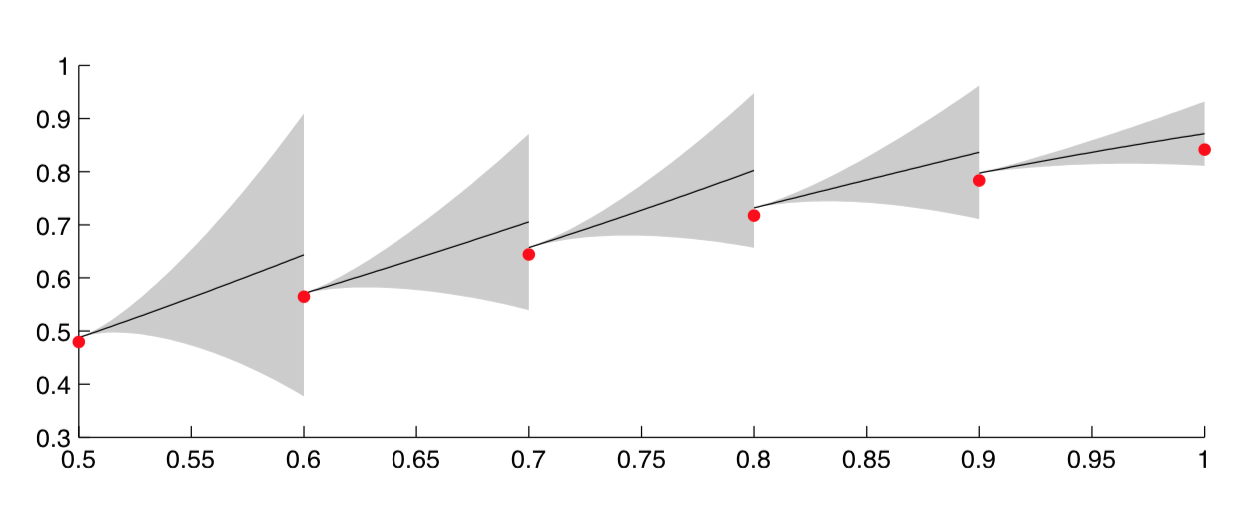
\includegraphics[width=0.75\textwidth]{gpar.png}
    \caption{Successive simulation of the GP-AR model}
    \label{fig:gparDiag}
\end{figure}


GP-AR and GP-ARX models can be understood as probabilistic simulation models. In \cref{fig:gparDiag} we can 
see a schematic illustration of such an iterative probabilistic system. To better understand \cref{fig:gparDiag}, 
we formalise the time stepping of the GP-AR model.

The iterative dynamics of GP-AR is captured in \cref{eq:gpARInit,eq:gpARProp}. The initial seed of the process is the 
system trajectory from time step $0$ to time step $p-1$ which is sampled from a standard multivariate Gaussian distribution. At each time step $t$, $y_t$ conditional to the system trajectory $\mathbf{y}_{t-1}$ is sampled 
from a Gaussian distribution (\cref{eq:gpARProp}) whose mean and covariance are calculated by appropriately 
conditioning the joint distribution in \cref{eq:systemTrajProb} and constructing the system state 
$\mathbf{x}_t$ and design matrix $\mathbf{X}_{t-1}$.     
%
\begin{align}
    (y_0, \cdots, y_{p-1}) &\sim \mathcal{N}(\mathbf{0}, \mathbf{I}) \label{eq:gpARInit}\\
    y_t \rvert \mathbf{y}_{t-1} &\sim \mathcal{N}(\bar{m}_t, \bar{\sigma}_{t}^2) \label{eq:gpARProp}
\end{align}
%
\begin{equation}\label{eq:postGPAR}
    \begin{aligned}
        \bar{m}_t &= m(\mathbf{x}_t) + 
        \mathbf{k}_{t}^{\intercal}\mathbf{K}_{t}^{-1}\left( \mathbf{y}_t - m(\mathbf{X}_{t-1}) \right) \\
        \bar{\sigma}^{2}_{t} &= K(\mathbf{x}_t, \mathbf{x}_t) - 
        \mathbf{k}_{t}^{\intercal} \mathbf{K}_{t}^{-1} \mathbf{k}_{t}
    \end{aligned}
\end{equation}
%
In \cref{eq:postGPAR}, the mean and variance of the conditional distribution of $y_t \rvert \mathbf{y}_{t-1}$ are 
computed, where $\mathbf{K}_{t} = [K(\mathbf{X}_{t-1}, \mathbf{X}_{t-1})]_{(t-p) \times (t-p)}$ is the 
covariance matrix computed between each pair of rows of $\mathbf{X}_{t-1}$ and 
$\mathbf{k}_{t} = [K(\mathbf{x}_t, \mathbf{X}_{t-1})]_{1 \times (t-p)}$ is the cross covariance matrix computed 
between the input features $\mathbf{x}_t$ and each row of the $\mathbf{X}_{t-1}$.

\subsection*{Relationship with Time Series Models : $\mathrm{AR}(p)$}

Due to the abstract nature of GPs, they generalize common time series models. For example, consider 
$\mathrm{AR}(p)$, the family of discrete auto-regressive time series models shown in \cref{eq:ARp,eq:ARpNoise}. 
At each time step, the systems state $y_t$ is determined by a linear combination of $p$ previous system states 
$y_{t-1}, \cdots, y_{t-p}$ plus Gaussian noise.  
%
\begin{align}
    y_t &= \sum^{p}_{k = 1}{\beta_{k}y_{t-k}} + z_t \label{eq:ARp} \\
    z_t &\sim \mathcal{N}(0, \sigma^{2}_{\varepsilon})\label{eq:ARpNoise}
\end{align}
%
We can write \cref{eq:ARp,eq:ARpNoise} in probabilistic form as: 
\begin{equation*}
    y_t \rvert y_{t-1}, \cdots, y_{t-p} \sim \mathcal{N}(\sum^{p}_{k = 1}{\beta_{k}y_{t-k}}, \sigma^{2}_{\varepsilon})
\end{equation*}
%
We can see that the GP-AR model family contains the $\mathrm{AR}(p)$ model in \cref{eq:ARp} as a special case. 
By setting $m(\mathbf{x}_t) = \sum^{p}_{k = 1}{\beta_{k}Y_{t-k}}$ and 
$K(\mathbf{x}_t, \mathbf{x}_s) = \sigma^2_{\varepsilon}\delta(\mathbf{x}_t, \mathbf{x}_s)$, where $\delta(.,.)$ 
is the Dirac delta function, we obtain the conditional probability density of the random variable 
$y_t \rvert y_{t-1}, \cdots, y_{t-p}$ described above. \cite{roberts2013gaussian} note that the $\mathrm{AR}(p)$ 
process is also equivalent to an explicit time GP model having $m(t) = \mathbb{E}[y(0)]$ and a Mat\'{e}rn 
covariance function
%
\begin{equation*}
    K(t, s)=\sigma ^{2}{\frac {2^{1-\nu }}{\Gamma (\nu )}}
    {\Bigg (}
        {\sqrt {2\nu }}{\frac {\rvert t - s \rvert}{\rho }}
    {\Bigg )}^{\nu }\mathcal{K}_{\nu }{\Bigg (}{\sqrt {2\nu }}{\frac {\rvert t - s \rvert}{\rho }}{\Bigg )}
\end{equation*}
%
with $\nu = p + \frac{1}{2}$, where $\Gamma(.)$ the gamma function, $\mathcal{K}_{\nu }(.)$ the modified 
Bessel function of the second kind, $\rho$ being the length scale and $\sigma^2$ the amplitude of $K(.,.)$.

The advantage of the implicit time GP-AR model over the explicit time GP model is that the GP-AR family 
can also simulate non-linear auto-regressive processes. This is because the kernel creates a Hilbert space 
$\mathcal{H}(\mathbb{C})$ spanned by a basis of non-linear orthogonal basis functions 
$\phi \in \mathcal{H}(\mathbb{C})$, such that the kernel can be decomposed 
\citep[sec.~4.3]{Rasmussen:2005:GPM:1162254} in the following manner.
%
\begin{equation*}
    K(\mathbf{x}_t, \mathbf{x}_s) = \sum^{\infty}_{i = 1}{\lambda_{i}\phi(\mathbf{x}_t) \bar{\phi(\mathbf{x}_s)}}
\end{equation*}
%
\citet[ch.~2]{Rasmussen:2005:GPM:1162254} also notes that \enquote{Gaussian process regression can be viewed as Bayesian linear regression with a possibly infinite number of basis functions}. We provide a simple example of how the GP-AR 
model can approximate the dynamics of a non-linear auto-regressive system.

\section*{Example: System Identification}

\begin{figure}[ht]
    \centering
    \noindent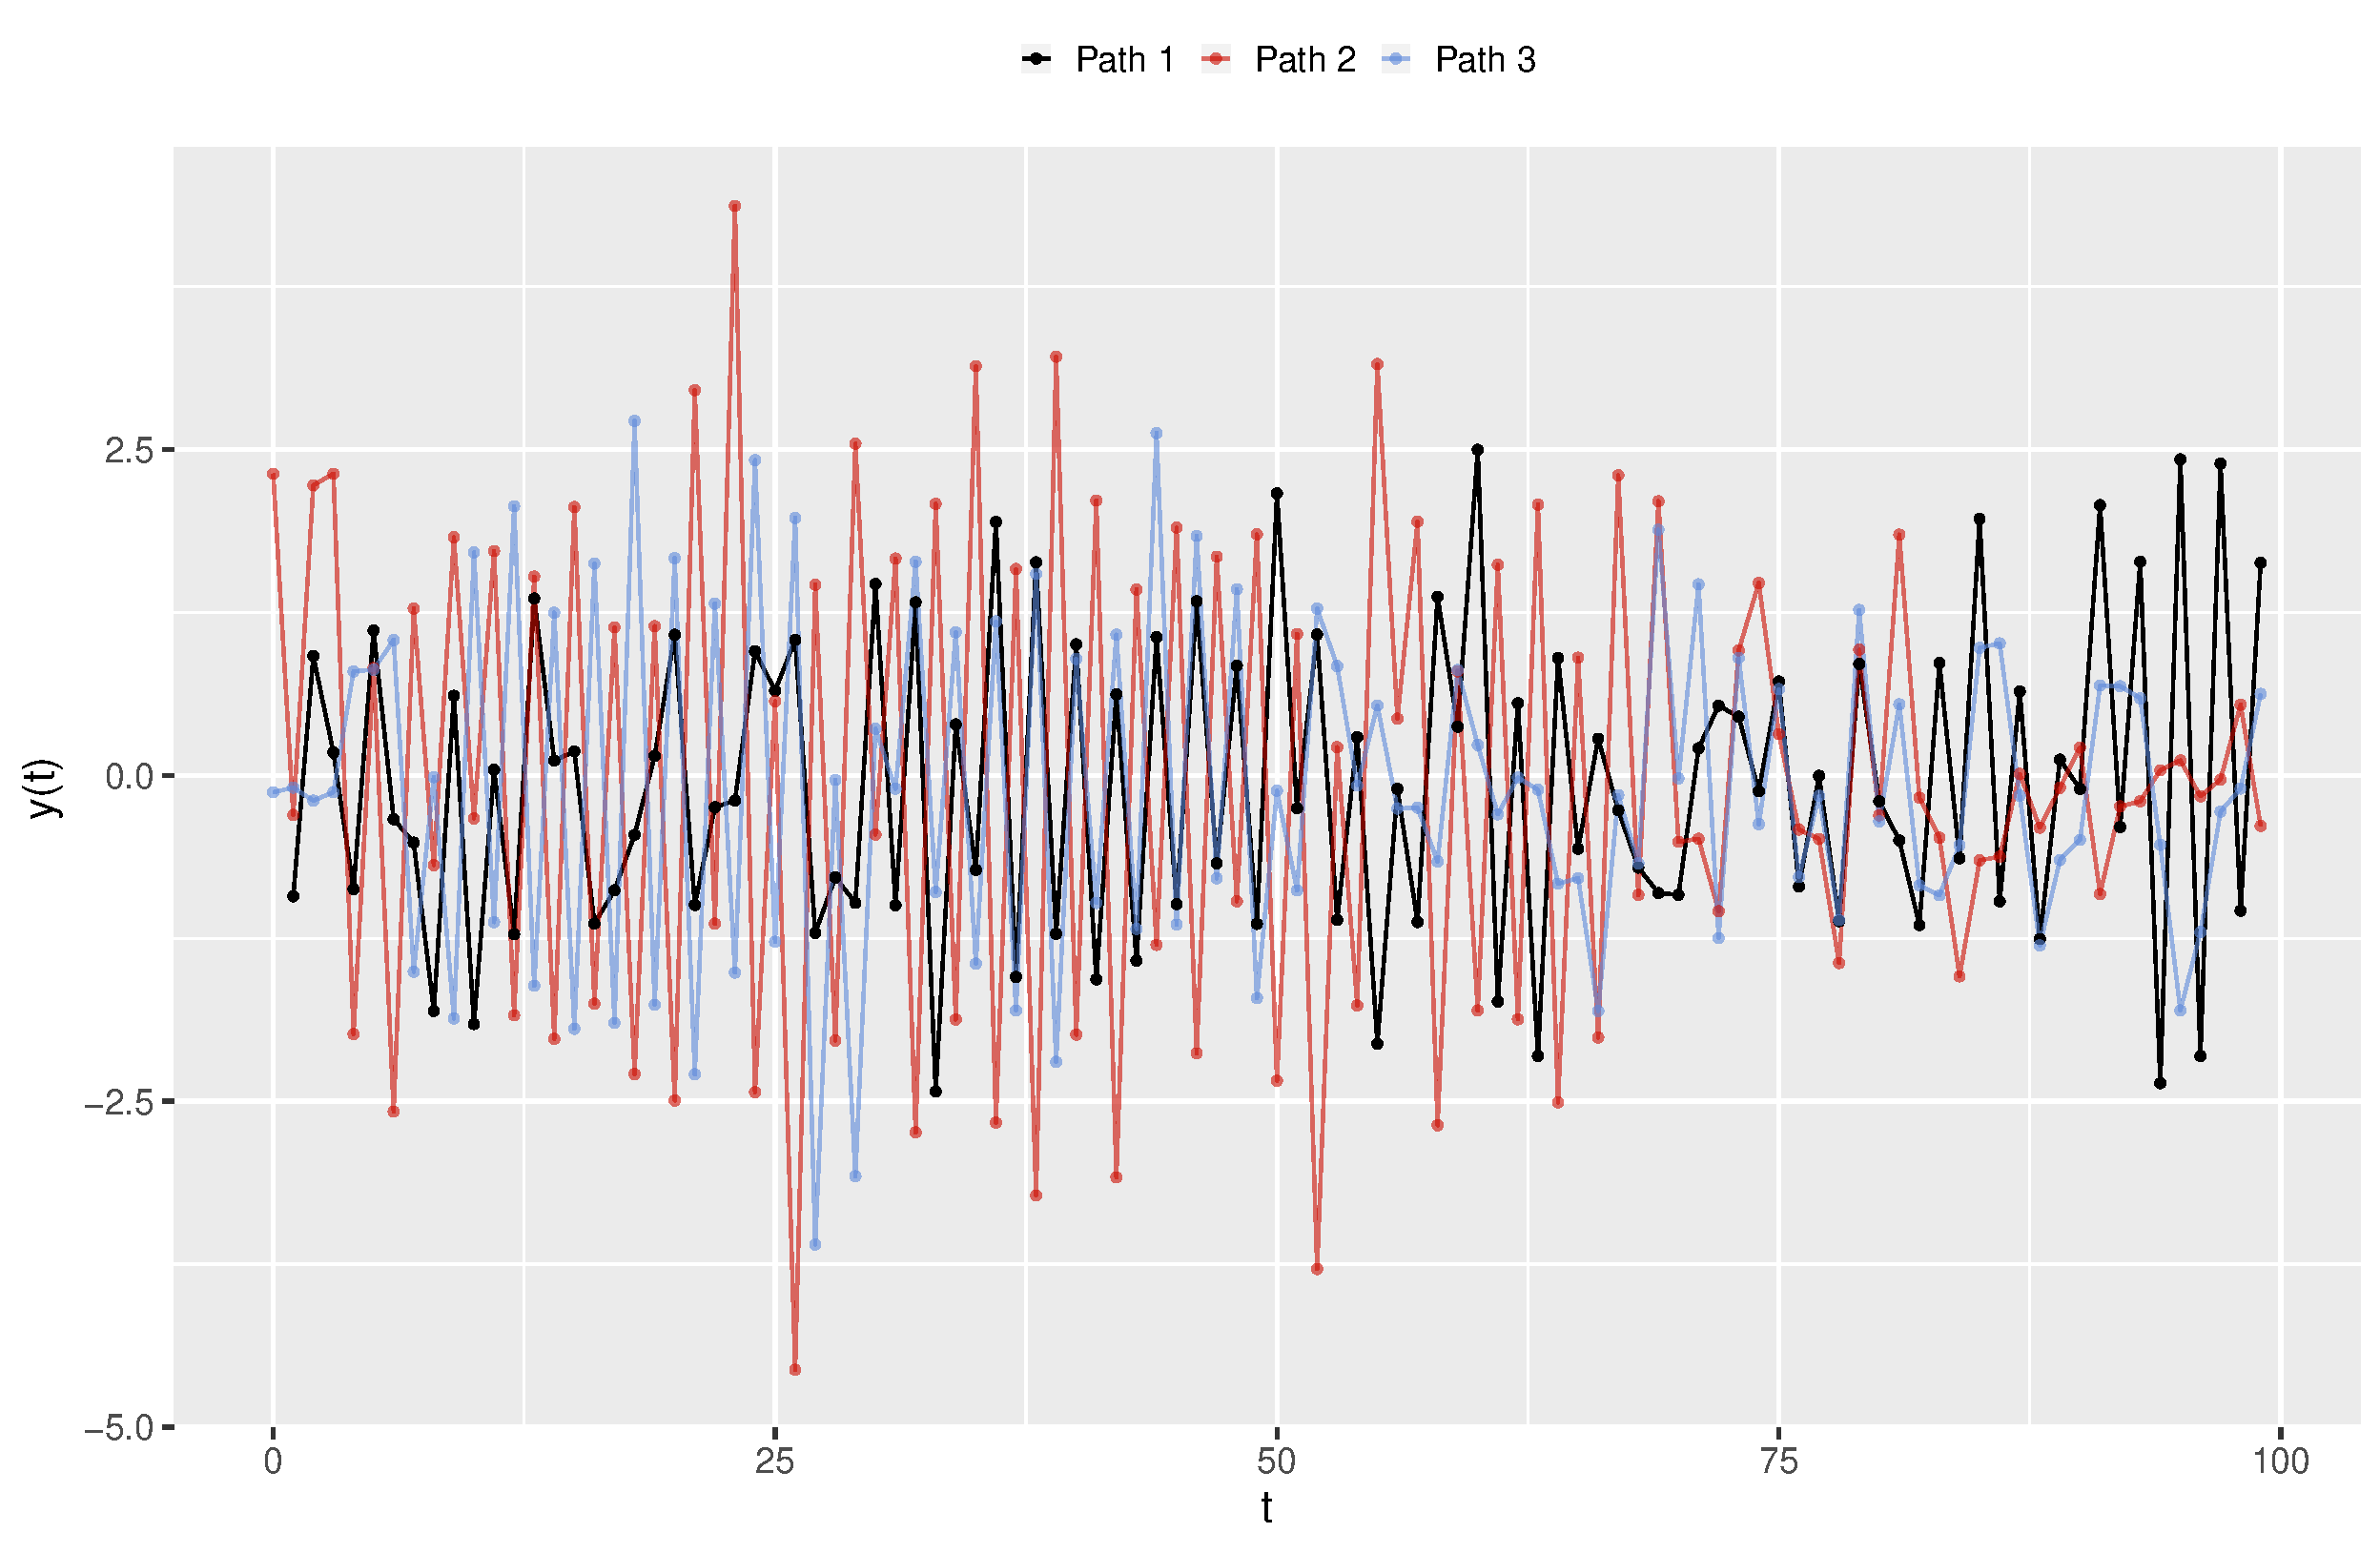
\includegraphics[width=\textwidth]{nar_samples.pdf}
    \caption{Samples drawn from non-linear autoregressive model in \cref{eq:narp}. 
    The path coloured in black is used partially ($t \leq 40$) in the training and the rest 
    as test data}
    \label{fig:narpSamples}
\end{figure}

Consider $y_t$, a quadratic auto-regressive system of order three, expressed below.
%
\begin{align}\label{eq:narp}
    y_0 &\sim \mathcal{N}(0, 1)\\
    \varepsilon &\sim \mathcal{N}(0, \sigma^{2}_{\varepsilon})\\
    y_t &= -0.05 y_{t-1} + 0.25 y_{t-2} - 0.63 y_{t-3} \\
        & - 4\times10^{-3} y^2_{t-1} - 0.02 y^{2}_{t-3} - 0.05 y^{2}_{t-2} \\ 
        & - 0.048 y_{t-2} y_{t-1} - 0.02 y_{t-1} y_{t-3} - 0.06 y_{t-2} y_{t-3} \\
        & + \varepsilon
\end{align}
%
The initial state $y_0$ is sampled from the standard Gaussian distribution. At time $t$, $y_t$ is determined 
by a series expansion up to degree two, of monomials constructed from $y_{t-1}, y_{t-2}, y_{t-3}$, plus Gaussian 
distributed noise $\varepsilon$.

Using the sampling procedure described above, we construct $10$ sample paths of temporal length $100$ for 
training and testing the GP-AR model (some of them shown in \cref{fig:narpSamples}). The portion $t > 40$ of the 
black path in \cref{fig:narpSamples} is reserved for model evaluation while its earlier segment as well 
as all other sample paths are retained for model training.  

We construct a GP-AR model with input 
$\mathbf{x}_t = \begin{bmatrix} y_{t-1}\\ y_{t-2}\\ y_{t-3}\\ \end{bmatrix}$, as
%
\begin{equation*}
    \begin{aligned}
        y_t &= f(\mathbf{x}_t) + \epsilon \\
        f(\mathbf{x}_t) &\sim \mathcal{GP}(m(\mathbf{x}_t), K(\mathbf{x}_t, \mathbf{x}_s)) \\
        \epsilon &\sim \mathcal{N}(0, \sigma_{\epsilon}^{2})
    \end{aligned}
\end{equation*}
%
with mean and covariance functions are defined as
\begin{equation*}
    \begin{aligned}
        m(\mathbf{x}_t) &=  -0.05 y_{t-1} + 0.25 y_{t-2} - 0.63 y_{t-3}\\
        K(\mathbf{x}_t, \mathbf{x}_s) &= \sigma^2 
        \exp \left(-\frac{1}{2} \frac{\rvert \rvert \mathbf{x}_t - \mathbf{x}_s \rvert \rvert ^2}{l^2} \right)
    \end{aligned}
\end{equation*}
where the kernel and noise parameters are initialised as follows $\sigma^2 = 2$, $l = 1$, 
$\sigma_{\epsilon}^{2} = 0.5$. In \cref{fig:gparPrior}, we show some samples drawn from this GP-AR prior.
%
\begin{figure}[ht]
    \centering
    \noindent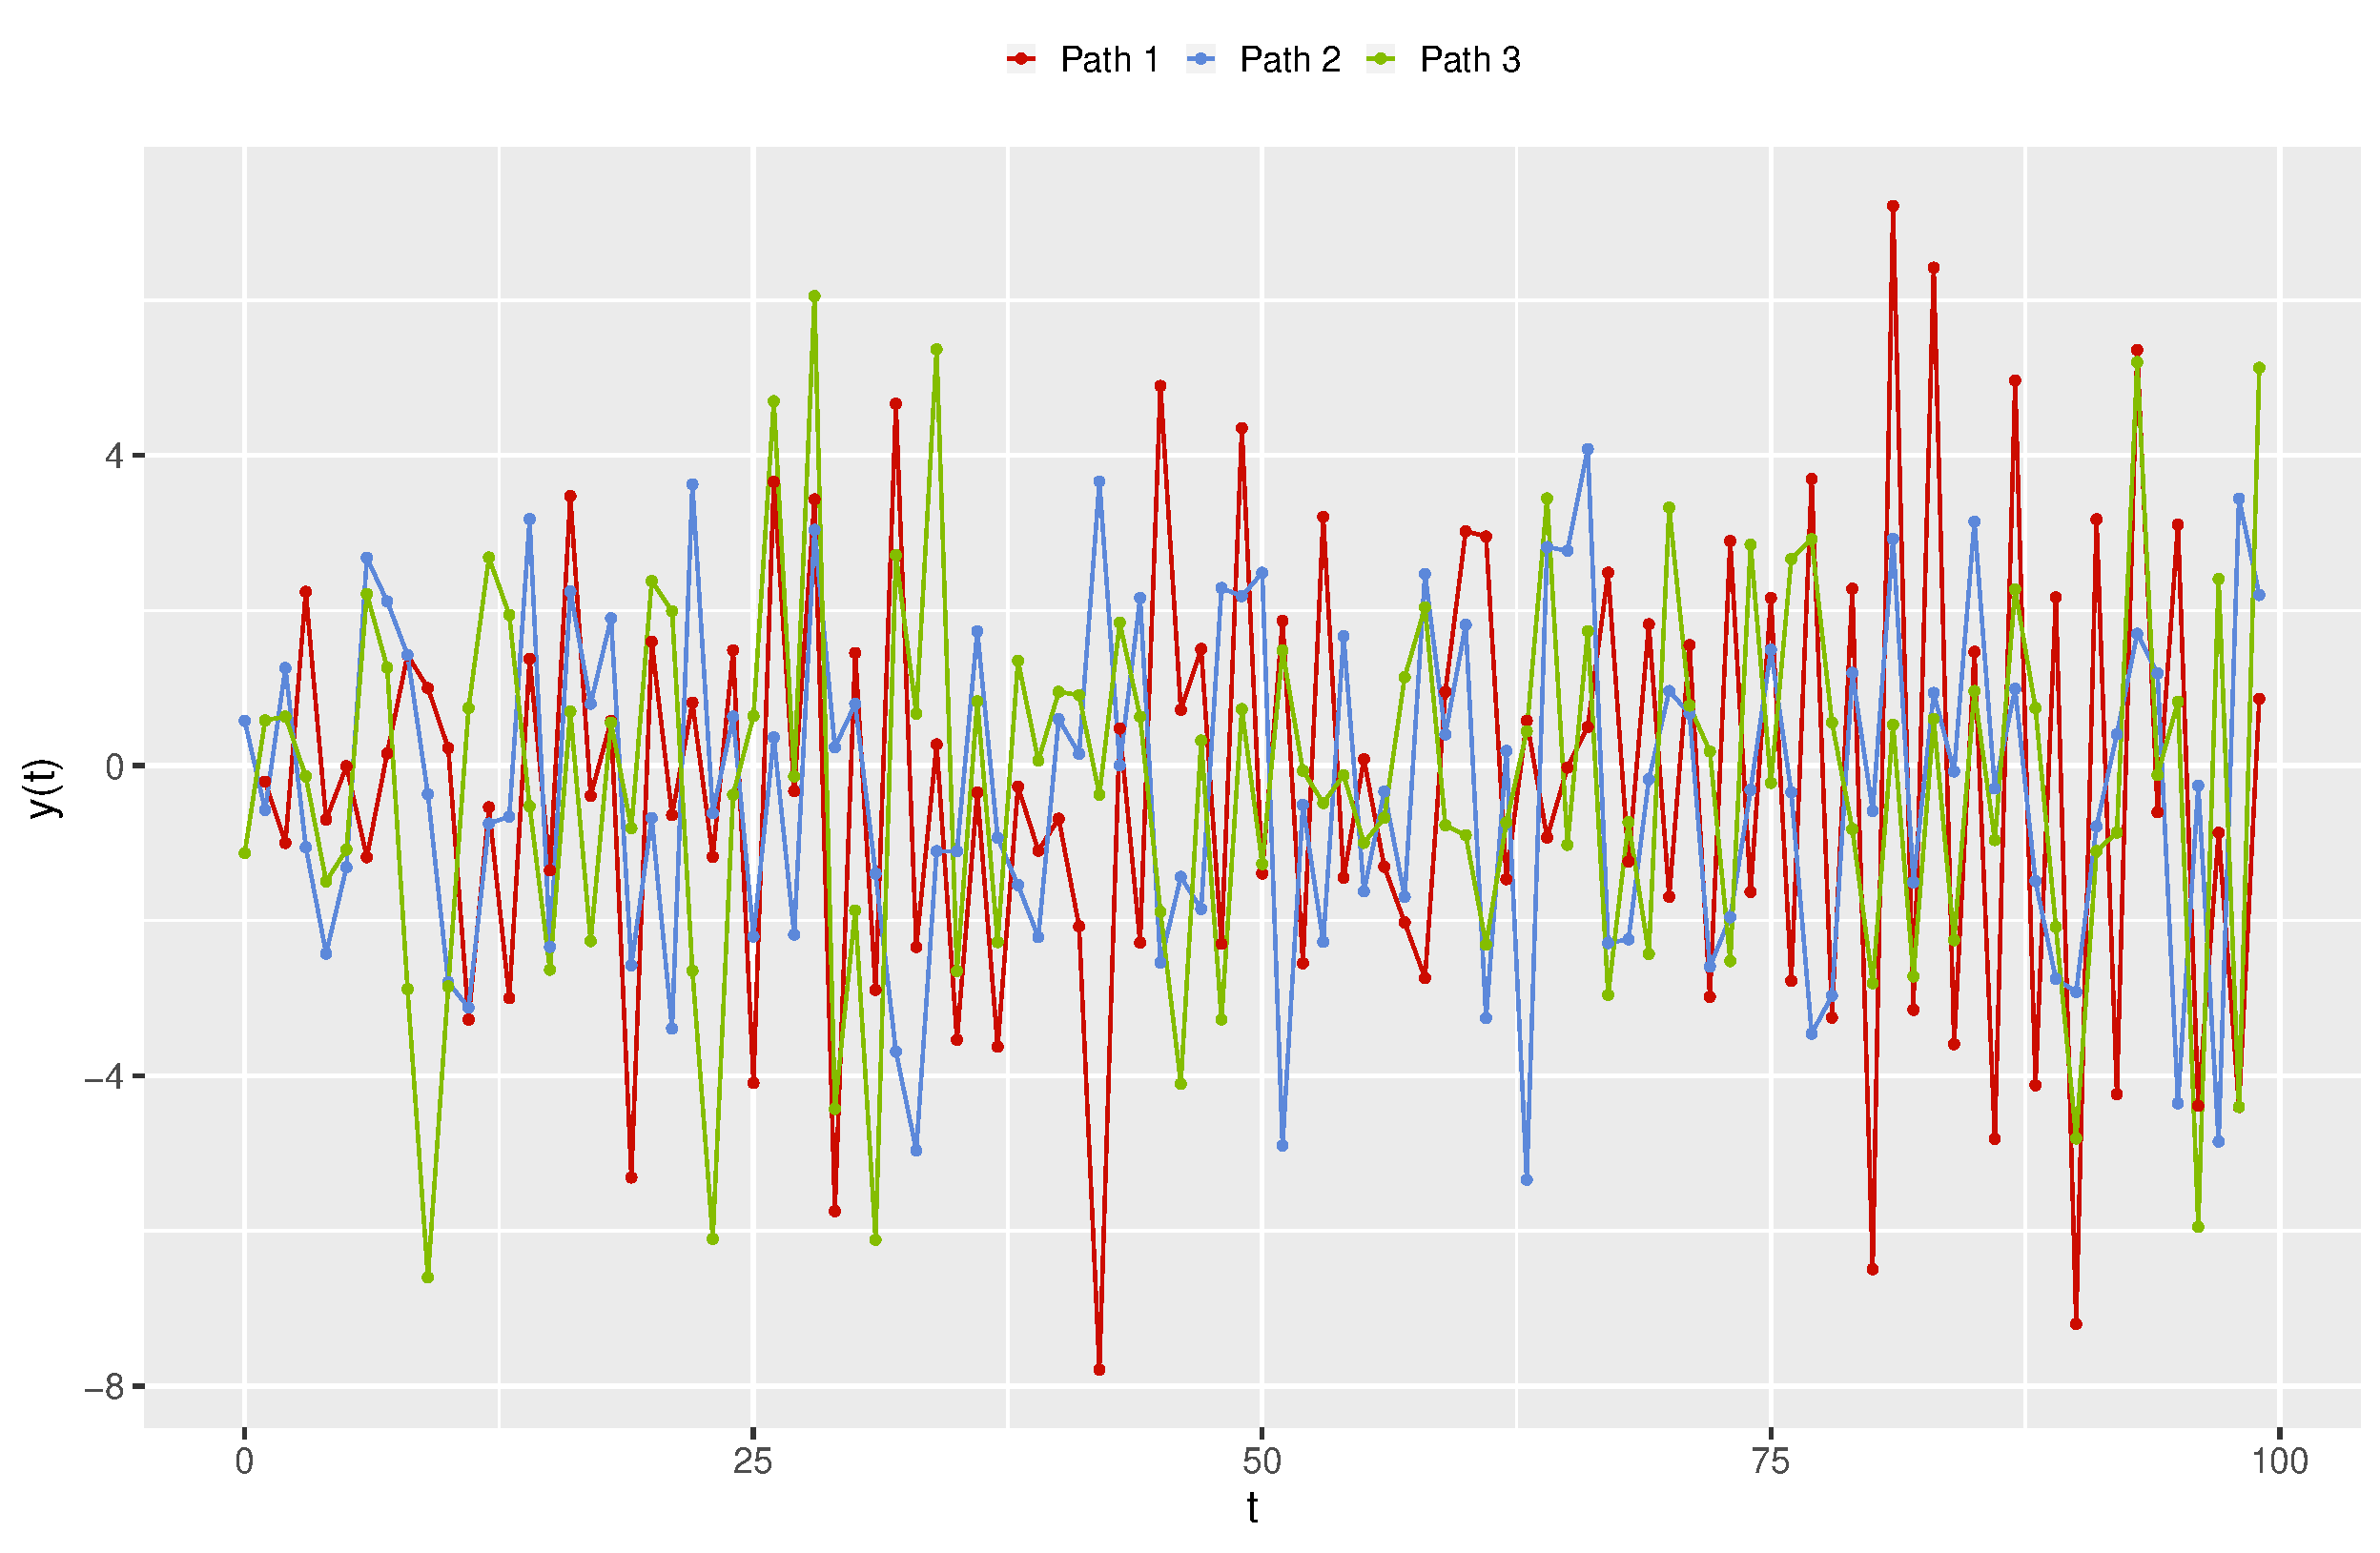
\includegraphics[width=\textwidth]{gp_nar_prior.pdf}
    \caption{Prior samples drawn from a GP-AR model (\cref{eq:gpARInit,eq:gpARProp}) with an squared exponential kernel.}
    \label{fig:gparPrior}
\end{figure}
%
During the training procedure, the model's hyper-parameters are selected using the CSA procedure described in 
\cref{sec:gpModelSelection}. After choosing the model hyper-parameters, the model is tested on the 
portion $t > 40$ of the black path in \cref{fig:narpSamples}. 

In \cref{fig:gparPost}, the posterior predictive distribution of the GP-AR model is used to generate one step ahead 
predictions with error bars. The GP-AR model is able to approximate the quadratic dynamics of \cref{eq:narp}, 
although the prior mean function $m(\mathbf{x}_t) =  -0.05 y_{t-1} + 0.25 y_{t-2} - 0.63 y_{t-3}$ only captures 
the linear components of \cref{eq:ARp}, the kernel enables modelling of the quadratic components.

\begin{figure}[ht]
    \centering
    \noindent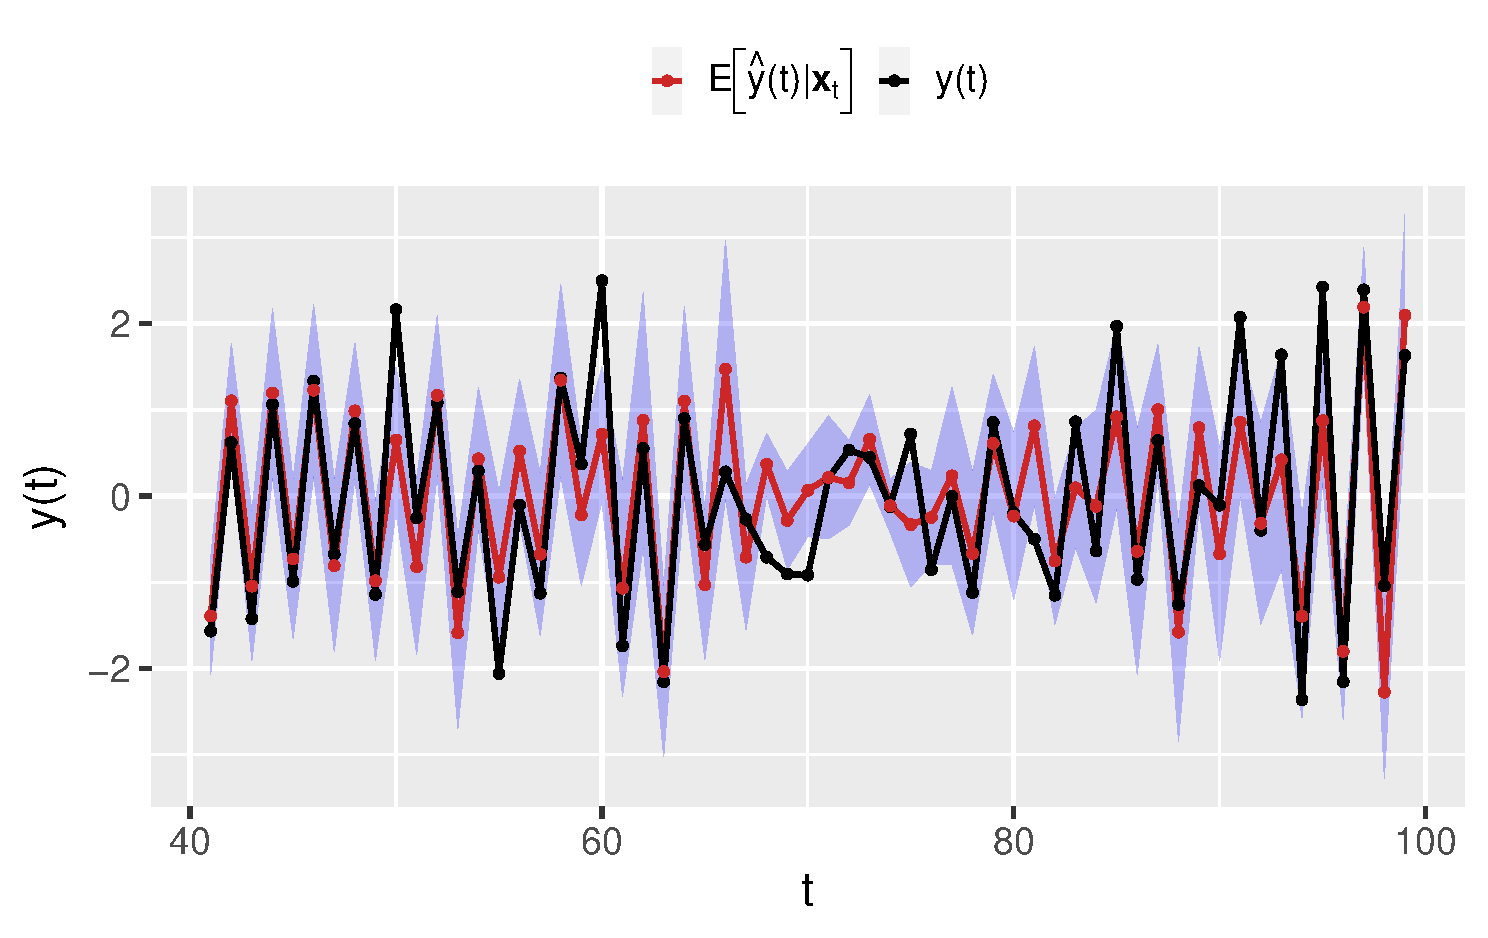
\includegraphics[width=\textwidth]{gp_nar_pred_partial.pdf}
    \caption{Predictions made by the GP-AR model, error bars shaded in blue.}
    \label{fig:gparPost}
\end{figure}

